\documentclass{article}

\usepackage{graphicx}
\usepackage{tikz}
\usepackage{tikzsymbols}
\usetikzlibrary{calc,patterns,shapes.geometric}
\pagestyle{empty}
\usepackage[margin=0pt]{geometry}
\geometry{papersize={14in,12in}}

\def\centerarc[#1](#2)(#3:#4:#5){\draw[#1] ($(#2)+({#5*cos(#3)},{#5*sin(#3)})$) arc (#3:#4:#5);}

\begin{document}
	\begin{figure}
		\centering
		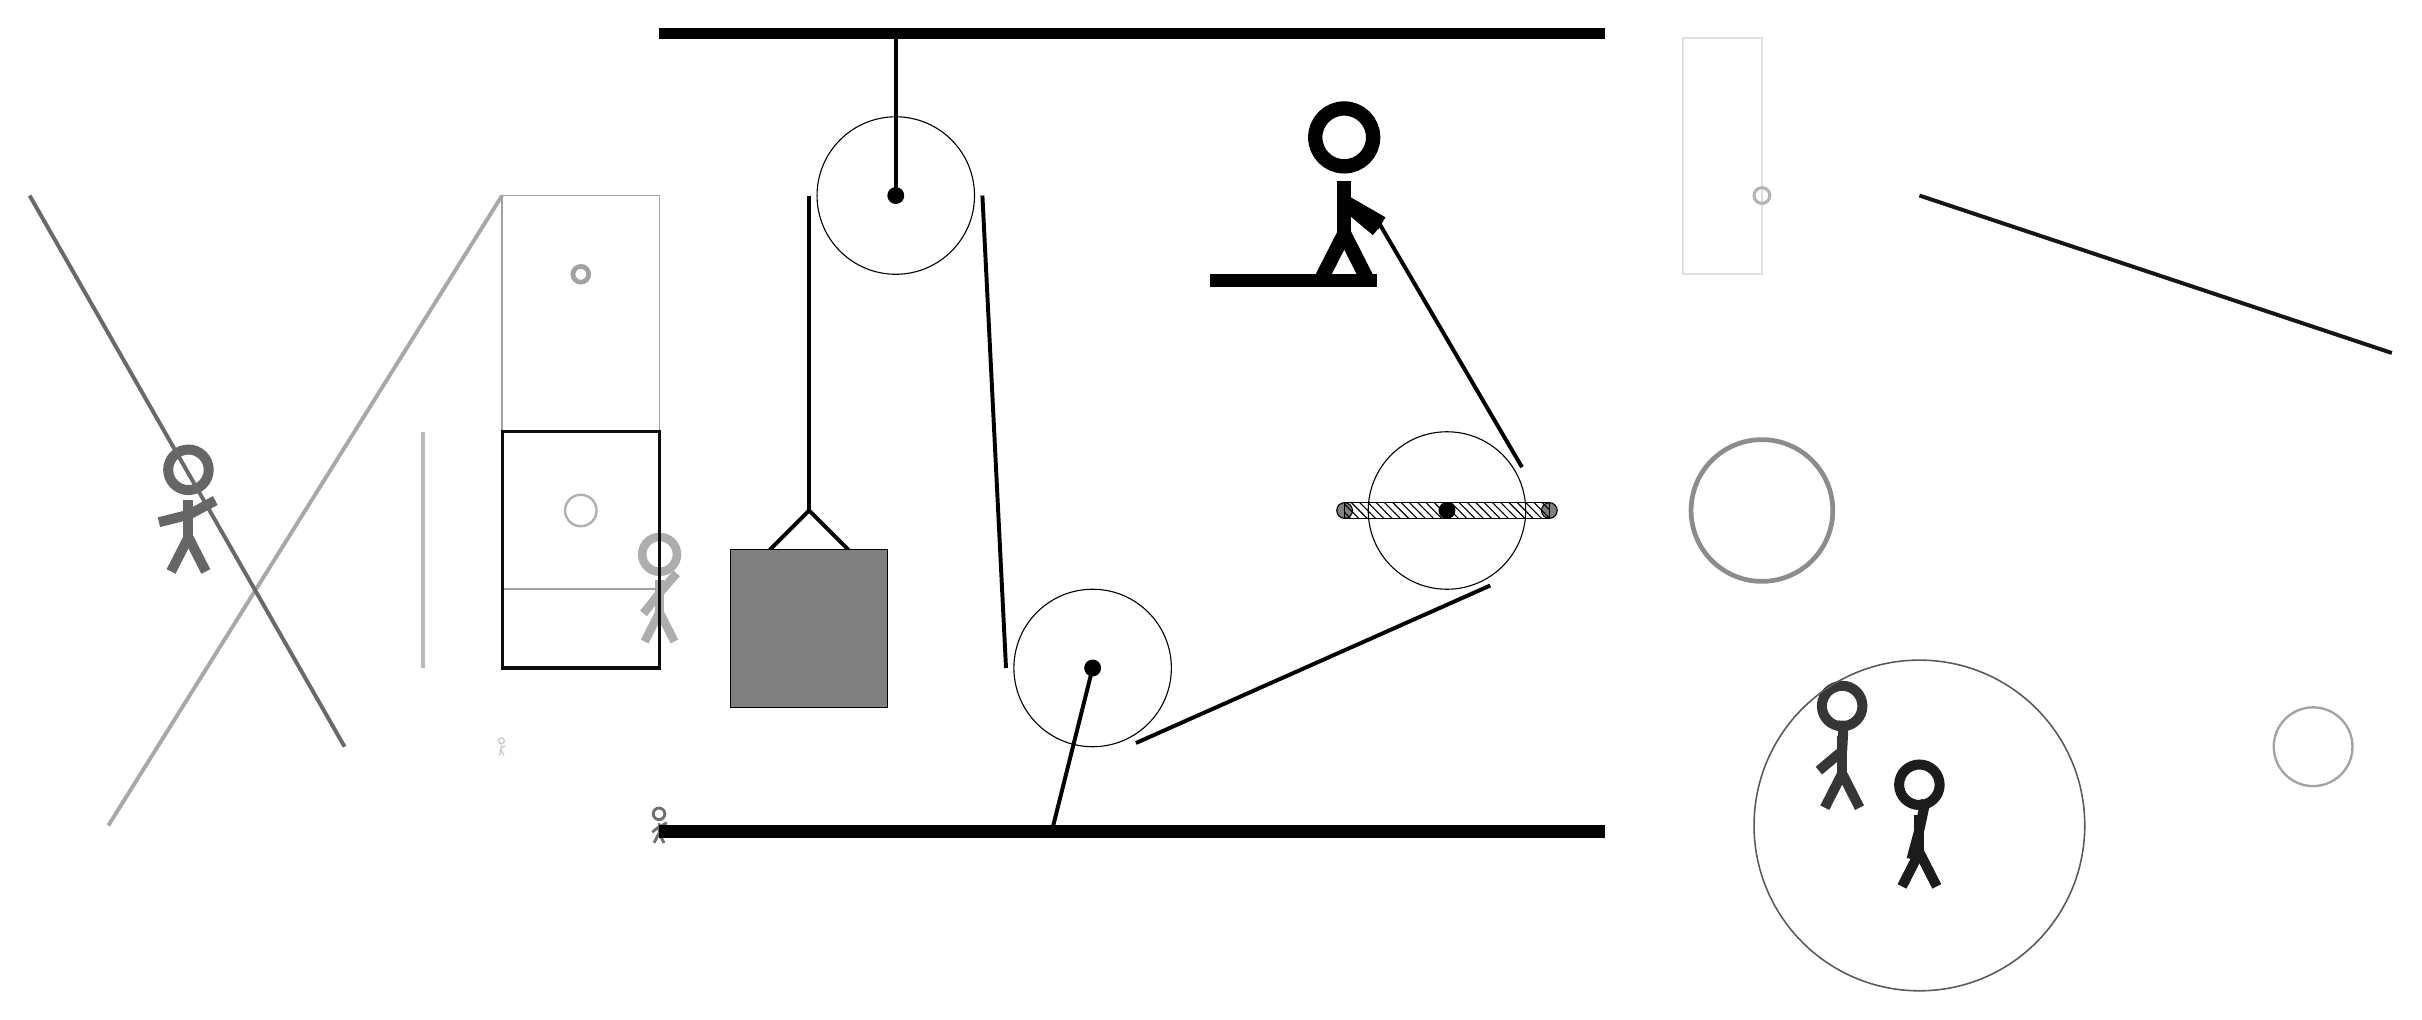
\begin{tikzpicture}
			%%%%% START %%%%%
			
			\draw[fill=black] (-2, 10) rectangle (10, 10.125);
			
			\draw (1, 8) circle (1);
			\draw[fill=black] (1, 8) circle (0.1);
			\draw[line width=0.5mm] (1, 10) -- (1, 8);
			
			\draw (3.5, 2.0) circle (1);
			\draw[fill=black] (3.5, 2.0) circle (0.1);
			\draw[line width=0.5mm] (3.5, 2.0) -- (3.0, 0);
			
			\draw[fill=white](8, 4.0) circle (1);
			\draw[fill=black] (8, 4.0) circle (0.1);
			\draw[fill=black!50] (9.3, 4.0) circle (0.1);
			\draw[fill=black!50] (6.7, 4.0) circle (0.1);
			\draw[pattern=north west lines, pattern color=black] (6.7, 4.1) rectangle (9.3, 3.9);
			
			\draw[line width=0.5mm](-0.6, 3.5) --  (-0.1, 4.0) -- (0.4, 3.5);
			\draw[fill=black!50] (-1.1, 3.5) rectangle (0.9, 1.5);
			
			\draw[line width=0.5mm, color=black!34](-4, 8) -- (-9, 0);
			
			\node[line width=0.6mm, color=black!60] at (-8, 4) {\Strichmaxerl[7][14][28]};
			\draw[line width=0.5mm, color=black!91](14, 8) -- (20, 6);
			\draw[line width=0.5mm, color=black!27](-5, 2) -- (-5, 5);
			\draw [line width=0.6mm, color=black!45](12, 4) circle (0.9);
			\node[line width=0.2mm, color=black!32] at (-2, 3) {\Strichmaxerl[6][52][49]};
			
			\draw[line width=0.2mm, color=black!36] (-4, 3) rectangle (-2, 8);
			\draw[line width=0.4mm, color=black!95] (-4, 2) rectangle (-2, 5);
			\node[line width=0.6mm, color=black!79] at (13, 1) {\Strichmaxerl[7][40][87]};
			\draw [line width=0.3mm, color=black!31](-3, 4) circle (0.2);
			
			\draw [line width=0.2mm, color=black!65](14, 0) circle (2.1);
			
			\node[line width=0.5mm, color=black!56] at (-2, 0) {\Strichmaxerl[2][39][26]};
			\draw[line width=0.2mm, color=black!12] (12, 7) rectangle (11, 10);
			
			\node[line width=0.6mm, color=black!20] at (-4, 1) {\Strichmaxerl[1][68][17]};
			\draw [line width=0.3mm, color=black!36](19, 1) circle (0.5);
			\draw [line width=0.6mm, color=black!37](-3, 7) circle (0.1);
			\draw [line width=0.4mm, color=black!29](12, 8) circle (0.1);
			\node[line width=0.3mm, color=black!89] at (14, 0) {\Strichmaxerl[7][75][78]};
			\draw[line width=0.5mm, color=black!59](-6, 1) -- (-10, 8);
			
			\draw[line width=0.5mm](-0.1, 8) -- (-0.1, 4.0);
			\centerarc[line width=0.5mm](1, 8)(180:0:1.1)
			\draw[line width=0.5mm](2.1, 8) -- (2.4, 2.0);
			\centerarc[line width=0.5mm](3.5, 2.0)(180:300:1.1);
			\draw[line width=0.5mm](4.05, 1.0474) -- (8.55, 3.0474);
			\centerarc[line width=0.5mm](8, 4.0)(300:390:1.1);
			\draw[line width=0.5mm](8.9526, 4.55) -- (7.05, 7.8);
			
			\node at (6.75, 8) {\Strichmaxerl[10][-220][-30]};
			\draw[fill=black] (5, 7) rectangle (7.1, 6.85);
			
			\draw[fill=black] (-2, 0) rectangle (10, -0.15);
			
			%%%%% END %%%%%
		\end{tikzpicture}
	\end{figure}	
\end{document}